\documentclass[11pt,letterpaper]{article}
\PassOptionsToPackage{hyphens}{url}
\usepackage[margin=.83in,top=.8in,bottom=.8in,headheight=15pt]{geometry}
\usepackage[T1]{fontenc}
\usepackage{lmodern,amsmath,amssymb,mathtools,bm,booktabs,array,graphicx,tikz}
\usetikzlibrary{arrows.meta,positioning,calc,decorations.pathreplacing,patterns}
\definecolor{ink}{HTML}{17344D}\definecolor{accent}{HTML}{087E8B}\definecolor{pale}{HTML}{EDF5F5}\definecolor{gold}{HTML}{AD6B19}
\providecommand{\dd}{\,\mathrm{d}}\providecommand{\R}{\mathbb{R}}
\providecommand{\E}{\mathbb{E}}\providecommand{\Var}{\operatorname{Var}}
\providecommand{\Cov}{\operatorname{Cov}}\providecommand{\diag}{\operatorname{diag}}
\providecommand{\norm}[1]{\left\lVert#1\right\rVert}
\providecommand{\abs}[1]{\left|#1\right|}
\usepackage{microtype,hyperref,fancyhdr,enumitem,amsthm,sectsty,needspace}
\allsectionsfont{\raggedright}
\hypersetup{colorlinks=true,linkcolor=ink,urlcolor=accent,pdfauthor={Zan Ahmad},pdftitle={NumPy arrays and linear inverse problems / Lecture notes}}
\setlength{\parindent}{0pt}\setlength{\parskip}{6pt}\linespread{1.07}
\setlist{itemsep=3pt,topsep=4pt,leftmargin=*}
\emergencystretch=2em\clubpenalty=10000\widowpenalty=10000
\pagestyle{fancy}\fancyhf{}\fancyhead[L]{\small Scientific Computing in Python}\fancyhead[R]{\small Lecture 3}
\fancyfoot[L]{\footnotesize Zan Ahmad}\fancyfoot[R]{\footnotesize\thepage}\renewcommand{\headrulewidth}{.3pt}
\newtheorem{proposition}{Proposition}\newtheorem{theorem}{Theorem}\newtheorem{lemma}{Lemma}
\theoremstyle{definition}\newtheorem{definition}{Definition}\newtheorem{example}{Example}
\numberwithin{equation}{section}
\begin{document}
{\small\scshape Scientific Computing in Python\hfill Lecture 3}\par\medskip
{\raggedright\hyphenpenalty=10000\exhyphenpenalty=10000\LARGE\bfseries\color{ink} NumPy arrays and linear inverse problems\par}\medskip
{\small Lecture notes}\par\bigskip
A detector converts a mixture into a set of signals. Recovering the mixture from the signals leads to a linear system. This example gives array dimensions a physical interpretation and separates three operations that look similar in code: multiplying entries, taking dot products, and solving equations.

\section{The observation matrix}
\hypertarget{note-the-observation-matrix}{}\label{note:the-observation-matrix}
{\small \href{slides.html\#frame=the-observation-matrix\&step=1}{Slides for this section}}\par
Let $c_A,c_B$ denote two concentrations and let $y_1,y_2$ denote detector signals. Calibration specifies the signal produced per unit concentration. Arranging those coefficients in rows gives one equation per detector. The model assumes additive responses and fixed calibration coefficients over the range considered.

\[
y=Ac,\qquad A=\begin{pmatrix}1&0.25\\0.20&1.20\end{pmatrix},\quad c=\begin{pmatrix}c_A\\c_B\end{pmatrix}.
\]

\[
y_1=c_A+0.25c_B,\qquad y_2=0.20c_A+1.20c_B.
\]

\subsection*{Matrix entries and units}
$A_{ij}$ is the response of detector $i$ to one concentration unit of constituent $j$.

\[
[A_{ij}]=\frac{\text{signal}}{\text{concentration}},\qquad [Ac]=\text{signal}.
\]
The row and column meanings are part of the model.
\section{Rows of observations}
\hypertarget{note-rows-of-observations}{}\label{note:rows-of-observations}
{\small \href{slides.html\#frame=rows-of-observations\&step=1}{Slides for this section}}\par
Suppose the concentration vectors are stored as rows of a matrix $C$. A single column-vector equation $y=Ac$ becomes $y^{\mathsf T}=c^{\mathsf T}A^{\mathsf T}$ after transposition. Stacking such rows gives $Y=CA^{\mathsf T}$. This explains the transpose in the implementation; it is determined by the storage convention.

\[
C\in\R^{n\times2},\quad A\in\R^{2\times2},\quad Y=CA^{\mathsf T}\in\R^{n\times2}.
\]

\[
Y_{ri}=\sum_{j=1}^{2}C_{rj}A_{ij}.
\]

\subsection*{Array multiplication}
\begin{minipage}{\linewidth}
\begin{verbatim}
Y = C @ A.T
\end{verbatim}
\end{minipage}

\texttt{@} contracts the shared index. Entrywise \texttt{C*A} is a different operation and need not even have compatible shapes.
\section{Solving the calibration equations}
\hypertarget{note-solving-the-calibration-equations}{}\label{note:solving-the-calibration-equations}
{\small \href{slides.html\#frame=solving-the-calibration-equations\&step=1}{Slides for this section}}\par
The determinant of this calibration matrix is $1.15$, so the two detector equations determine a unique concentration vector in exact arithmetic. A numerical solver applies a factorization of the matrix. Forming an explicit matrix inverse is unnecessary for solving a single system and generally adds work.

\[
\det A=1(1.20)-0.25(0.20)=1.15\ne0.
\]

\begin{minipage}{\linewidth}
\begin{verbatim}
c_hat = np.linalg.solve(A, y)
residual = A @ c_hat - y
\end{verbatim}
\end{minipage}

\subsection*{Elimination by hand}
Subtract $0.20$ times the first detector equation from the second:
\[
1.15c_B=y_2-0.20y_1.
\]

Then $c_A=y_1-0.25c_B$. The numerical solve carries out equivalent linear algebra.
\begin{center}\begin{minipage}{.98\linewidth}\centering
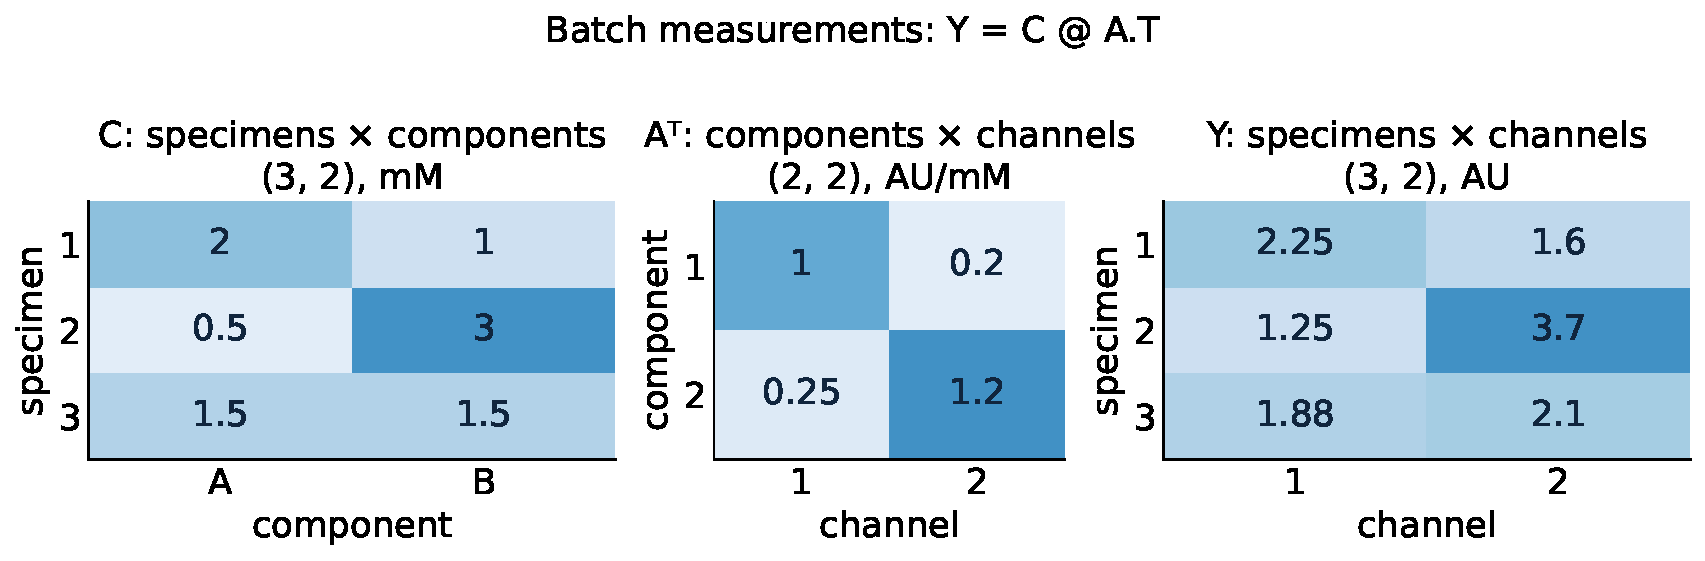
\includegraphics[width=.96\linewidth,height=.57\textheight,keepaspectratio]{presentation-figures/mixture-shapes.pdf}\par\smallskip
{\small Original synthetic concentration table, calibration transpose and detector signals. Entries are shown explicitly; each matrix uses its own shading scale.}
\end{minipage}\end{center}
\section{Residual and reconstruction error}
\hypertarget{note-residual-and-reconstruction-error}{}\label{note:residual-and-reconstruction-error}
{\small \href{slides.html\#frame=residual-and-reconstruction-error\&step=1}{Slides for this section}}\par
The residual measures how closely the computed concentrations satisfy the supplied detector equations. Reconstruction error compares them with the true concentrations, if those are known. These are different quantities. An error in the measured signal changes the system being solved and can produce a nearly zero residual together with a large concentration error.

\[
r=A\widehat c-y,\qquad e=\widehat c-c_{\rm true}.
\]

If $y=Ac_{\rm true}+\delta y$ and $r=0$, then
\[
Ae=\delta y.
\]

\subsection*{A residual scaled to the problem}
A dimensionless residual measure is
\[
\eta=\frac{\|A\widehat c-y\|_2}{\|A\|_2\|\widehat c\|_2+\|y\|_2}.
\]

A small $\eta$ supports the algebraic solve. It does not establish accurate calibration or accurate observations.
\section{Conditioning and redundant detectors}
\hypertarget{note-conditioning-and-redundant-detectors}{}\label{note:conditioning-and-redundant-detectors}
{\small \href{slides.html\#frame=conditioning-and-redundant-detectors\&step=1}{Slides for this section}}\par
For a nonsingular matrix, the condition number $\kappa_2(A)=\|A\|_2\|A^{-1}\|_2$ measures worst-case relative amplification of perturbations. Nearly proportional detector rows carry nearly the same information. Their small difference then determines a concentration component, making that component sensitive to noise.

\[
\delta c=A^{-1}\delta y,
\qquad
\frac{\|\delta c\|_2}{\|c\|_2}\leq\kappa_2(A)\frac{\|\delta y\|_2}{\|y\|_2}.
\]

The bound assumes $A$ is fixed and nonsingular.

\subsection*{Singular values}
If $A=U\Sigma V^{\mathsf T}$, then
\[
\kappa_2(A)=\frac{\sigma_{\max}}{\sigma_{\min}}.
\]

A small $\sigma_{\min}$ identifies a concentration direction that produces little signal.

For the relative perturbation bound, assume $c\ne0$ and $y\ne0$. If both the residual numerator and its normalization denominator vanish, report the exact zero residual separately rather than forming $0/0$.
\begin{center}\begin{minipage}{.98\linewidth}\centering
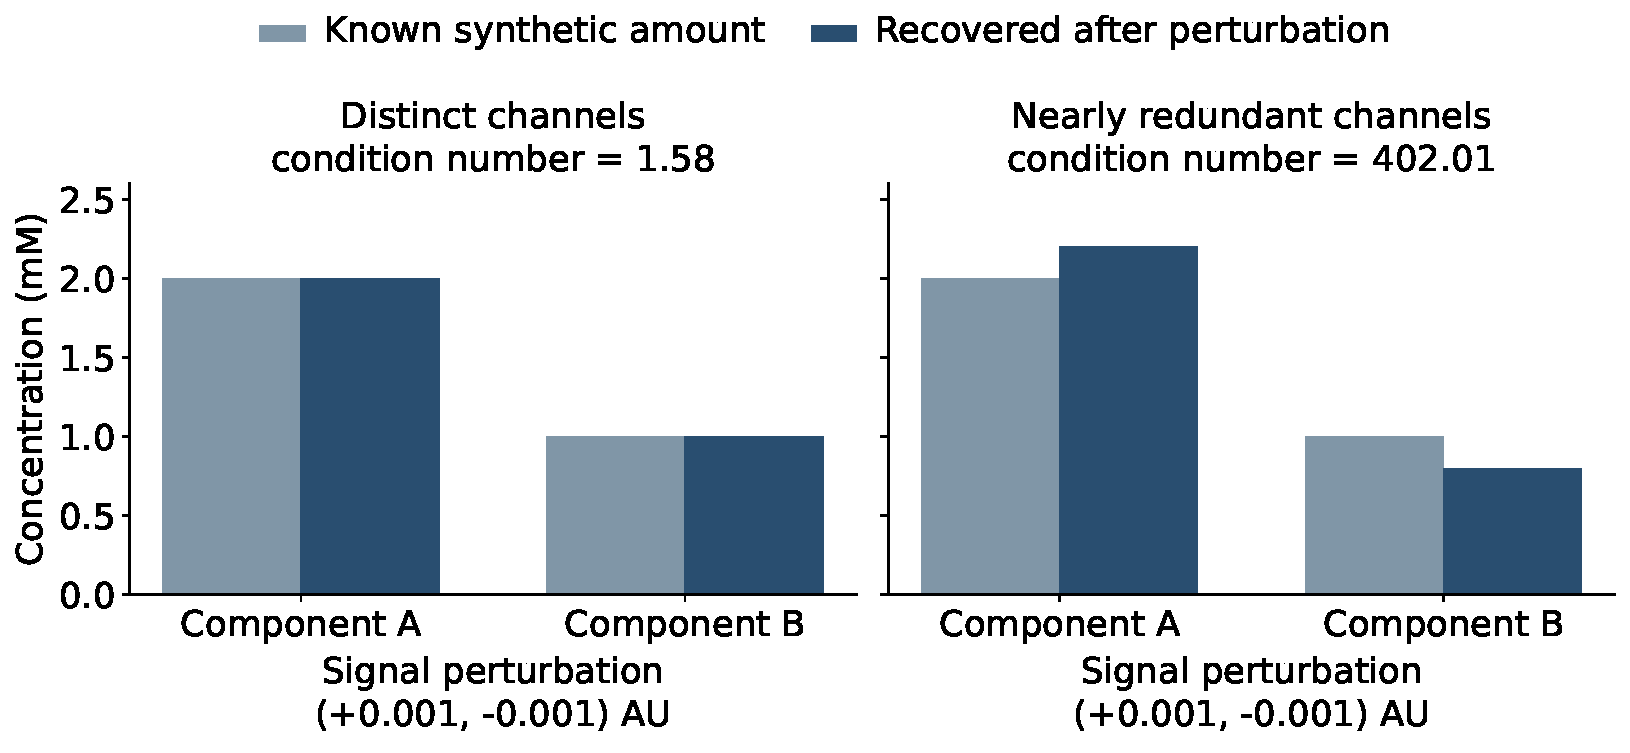
\includegraphics[width=.96\linewidth,height=.57\textheight,keepaspectratio]{presentation-figures/sensitivity.pdf}\par\smallskip
{\small Computed recovery for the same synthetic mixture and signal perturbation. Distinct channels have condition number about 1.58; nearly redundant channels about 402. Both residuals are close to rounding error.}
\end{minipage}\end{center}
\section{Batch solves and physical constraints}
\hypertarget{note-batch-solves-and-physical-constraints}{}\label{note:batch-solves-and-physical-constraints}
{\small \href{slides.html\#frame=batch-solves-and-physical-constraints\&step=1}{Slides for this section}}\par
For many signal vectors, pass the transposed observation table as multiple right-hand sides and transpose the solution back. Nonnegative concentrations may be required physically, but clipping a negative unconstrained solution does not solve the original equations or a specified constrained optimization problem. A constrained inverse model must state its objective and constraints explicitly.

\begin{minipage}{\linewidth}
\begin{verbatim}
C_hat = np.linalg.solve(A, Y.T).T
\end{verbatim}
\end{minipage}

This solves the same calibrated map for every row of observations.

\subsection*{A constrained alternative}
With noisy signals one may instead define
\[
\min_{c\geq0}\|Ac-y\|_2^2.
\]

The constraint changes the mathematical problem. Its residual is generally nonzero.
\bigskip
\section*{Exercises}
\par\noindent\begin{minipage}{\linewidth}
\subsection*{H3-1. A new calibration}
Two specimens have concentrations [1, 2] mM and [3, 0.5] mM. A new detector has response rows [2, 0.5] and [0.25, 1] AU/mM.

\textbf{a} State the shapes and axis meanings of C, A and Y.

\end{minipage}\par\medskip
\textbf{b} Calculate every detector signal without a library call.

\textbf{c} Write the matrix expression and one independent check.

\par\noindent\begin{minipage}{\linewidth}
\subsection*{H3-2. Two measurements that do not identify two amounts}
The response rows are [1, 1] and [2, 2] AU/mM. A specimen yields (3, 6) AU.

\textbf{a} Give two different nonnegative mixtures that fit the signals.

\end{minipage}\par\medskip
\textbf{b} Explain why the second channel does not remove the ambiguity.

\textbf{c} What would signals (3, 6.1) AU imply under the exact model, and what should the program report?

\par\noindent\begin{minipage}{\linewidth}
\subsection*{H3-3. Residual versus sensitivity}
A calibration has rows [1, 1] and [1, 1.02] AU/mM. The true amounts are (1, 2) mM. Add (+\allowbreak{}0.002, -0.002) AU to the two signals.

\textbf{a} Compute the unperturbed and perturbed signals.

\end{minipage}\par\medskip
\textbf{b} Recover the perturbed amounts by subtracting the two equations.

\textbf{c} Why can this answer have zero algebraic residual yet differ noticeably from the true mixture?

\par\noindent\begin{minipage}{\linewidth}
\subsection*{H3-4. Design a defensible check}
A colleague reports a detector calculation on 100 specimens. The program returns a table with shape (100, 2), including one negative recovered amount.

\textbf{a} Describe a unit check and a hand-calculation check before accepting the table.

\end{minipage}\par\medskip
\textbf{b} Describe a controlled perturbation experiment.

\textbf{c} Should the negative concentration be replaced by zero? Explain.

\section*{References}
\noindent\begin{minipage}{\linewidth}
Original Python Lecture 2. PDF pp. 30--43: array creation, shapes, products, solve and random seeds.

\url{https://zanahmad.com/files/scientific-python/Lecture_2__Intro_to_Python.pdf}
\end{minipage}\par\medskip
\noindent\begin{minipage}{\linewidth}
Original Python Lecture 3. PDF pp. 4--13: shapes, linear systems, least squares and floating-point comparisons.

\url{https://zanahmad.com/files/scientific-python/Lecture_3__Intro_to_Python.pdf}
\end{minipage}\par\medskip
Python source materials: Phillip Kerger (2023). Course adaptation and additional exposition: Zan Ahmad.

\end{document}
